\documentclass[11pt, oneside]{article}   	% use "amsart" instead of "article" for AMSLaTeX format
\usepackage{geometry}                		% See geometry.pdf to learn the layout options. There are lots.
\geometry{letterpaper}                   		% ... or a4paper or a5paper or ... 
%\geometry{landscape}                		% Activate for for rotated page geometry
%\usepackage[parfill]{parskip}    		% Activate to begin paragraphs with an empty line rather than an indent
\usepackage{graphicx}				% Use pdf, png, jpg, or epsß with pdflatex; use eps in DVI mode
								% TeX will automatically convert eps --> pdf in pdflatex		
\usepackage{amssymb}
\usepackage{url}
\usepackage{enumitem}
\usepackage{longtable}
\usepackage{comment}

\title{Comparison of JVM and Dalvik VM}
\author{Dainius Jocas}
%%\date{} % delete this line to display the current date

%%% BEGIN DOCUMENT
\begin{document}

\maketitle
\tableofcontents
\newpage

\begin{comment}
Structure of comparison:
\begin{enumerate}
  \itemsep0pt
  \item definition (goal, why to have one, advantages and disadvantages, safety)
  \item purpose (motivation) (sandboxing as a feature of VM)
  \item architecture
  \item implementation
  \item code support
  \item bytecode (.class vs. .dex files)
  \item memory / resource usage (GC)
  \item The large table goes to appendix.
  \item 
  \item internals of .class and .dex files and comparison
  \item licensing for the future.
  \item performance comparisons
\end{enumerate}


\begin{abstract}
The goal of this report is to compare Java Virtual Machine (JVM) and Dalvik virtual machine (DVM). To do this I'll compare file formats that are accepted by each virtual machines, also, briefly describe differences of stack- and registry-based machines and its implications, and review various optimizations used to construct the Dalvik VM executable comparing to JVM byte code and what improvements do they bring to the Android platform. 
\end{abstract}
\end{comment}

\begin{quotation}
\textit
{
Dalvik isn`t exactly a household word (at least in my country), and most people wouldn`t know a virtual machine if it hit them in the face, but when you tell them you were able to make their existing device work better -- run faster, use less battery -- they will actually take notice!
} (Dan Bornstein)\cite{website:dalvikjit2010}
\end{quotation}

\section*{Introduction}

The popularity of mobile devices is increasing very rapidly. It is considered that the most popular mobile platform for smartphones nowadays is Android\cite{website:popularplatform2012}. Here we can ask questions such as, why Android is so popular? Does Android meets the requirements for mobile platforms in the best way? To answer those questions we need to take a good look at the requirements for mobile computing and examine the Android approach to meet those requirement for mobile platform. 

\subsection*{Requirements for mobile platform}

Smartphone devices comparing to desktop or laptop cousins has various differences. Smartphones have to meet a whole bunch of restrictions that are not very important for desktops. The most important ones are:
\begin{itemize}
  \itemsep0em
  \item battery power
  \item passive cooling
  \item small form factor.
\end{itemize}
If we take a look at a typical smartphone characteristics: ARM CPU that runs at 500 MHz clock speed, with 128 MB of RAM, no swap space, limited external flash storage (usually NAND), and 1500 mAh battery capacity\cite{website:androiddalvikvm}, we can clearly see that we cannot simply use, for example, the same virtual machine as desktop computer with much greater capabilities, because the performance would be unacceptable and we would drain battery in matter of minutes.

\subsection*{Android approach to meet requirement for mobile platform}

Android is an open-source software stack for mobile phones and other devices\cite{website:androidphylosophy}. Android approach to meet requirements for mobile platform is to provide the whole software stack (e.g. Linux kernel, Java programming language, etc.) which is optimized exactly for mobile platform. 

\begin{figure}
  \center
  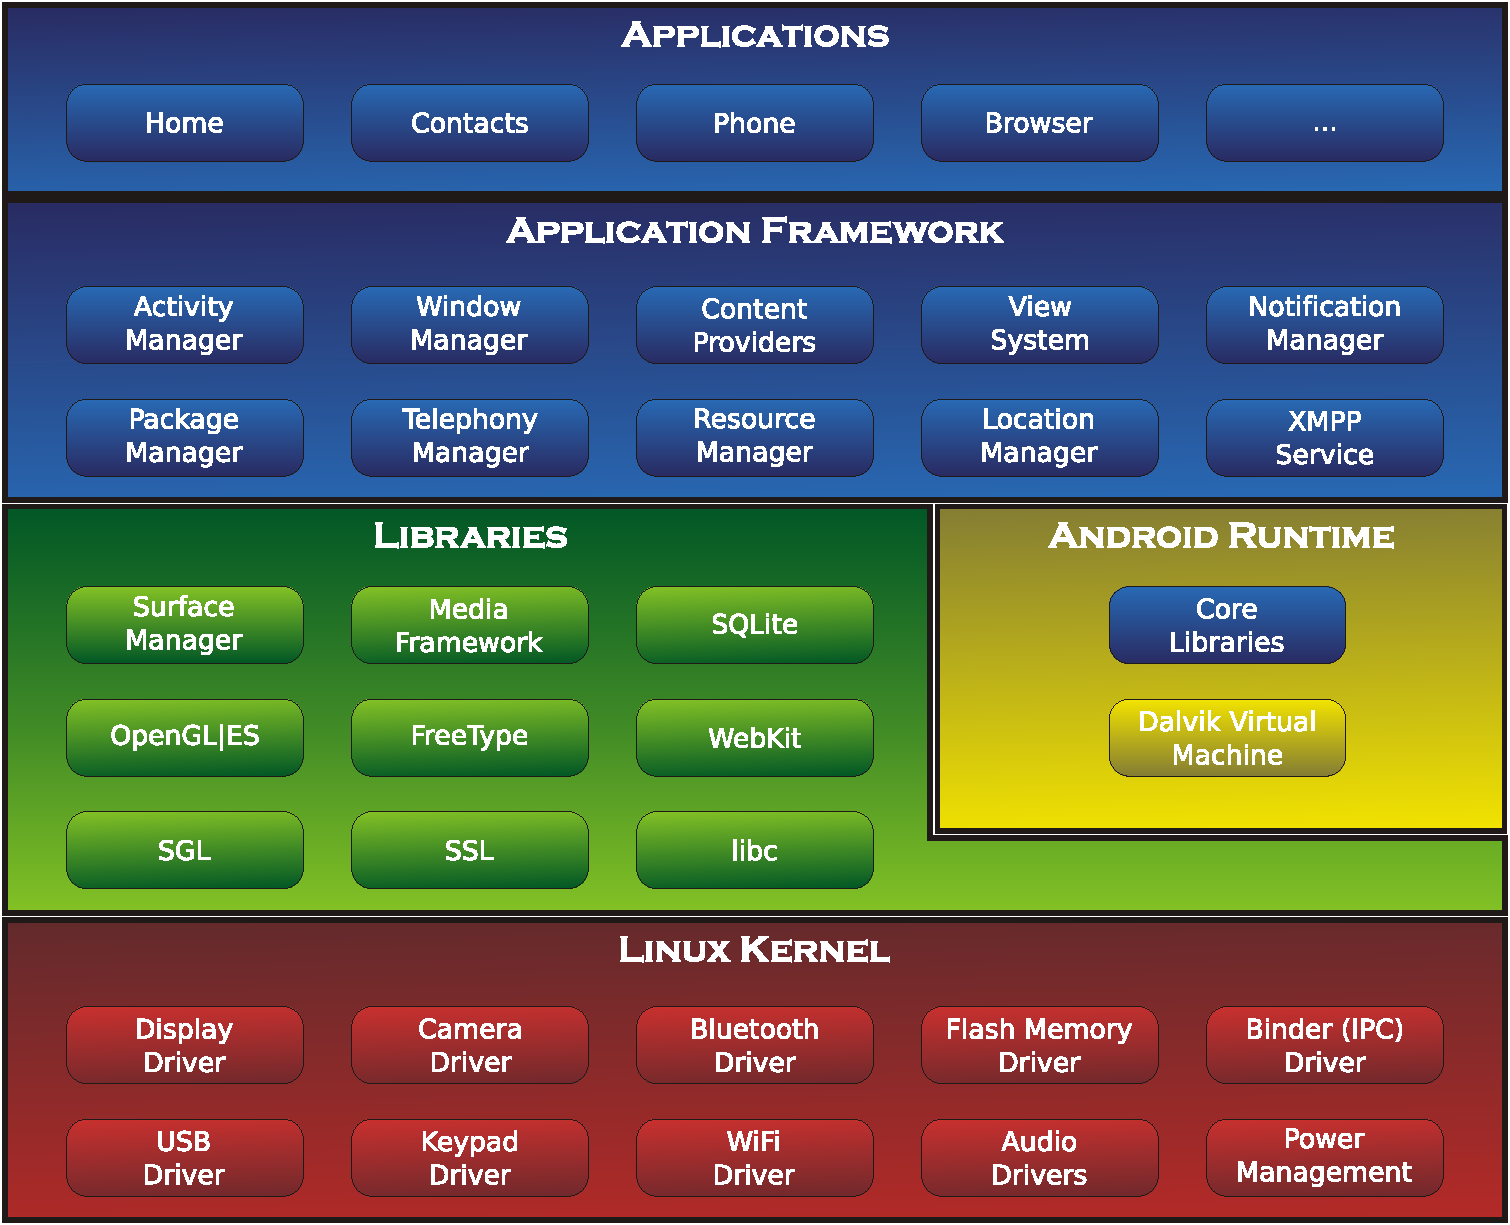
\includegraphics[width=0.7\textwidth]{./images/android_system_architecture.pdf}
  \caption{Android system architecture}
  \label{fig:figure1}
  \end{figure}

We can see that Android core developers are using technologies that already exist and are very popular. By using popular technologies Android platform can get the attention of lot of skilled developers which is probably the most important ingredient to make a successful mobile platform. 

\subsection*{The cornerstone for Android}

At the core (in terms of importance) of the Android platform we find a Dalvik virtual machine (DVM). Dalvik is the managed runtime used by applications and some system services on Android. Dalvik was originally created specifically for the Android project\cite{website:dalviktechnical}. DVM promises to run fast and have a small memory footprint on systems that has limited amount of memory and relatively slow CPU. This is exactly what is needed in the modern mobile platform.

DVM is an descendant of Java virtual machine (JVM). The rest of this report will discuss the main differences between the two virtual machines.

\section{Definition}

A virtual machine (VM) is a software implementation of a machine (i.e. a computer) that executes programs like a physical machine\cite{website:understandingjvminternals}. Basic VM parts are: a set of registers, a stack (optional), an execution environment, a garbage-collected heap, a constant pool, a method storage area, an instruction set.

In this section we explore definitions of the JVM and DVM and differences between the two.

% TODO(dainius) Ask Luis what exactly to write in the definition part?

\subsection{Definition of JVM as part of Java technology}

The name "Java" for programming language is said to originate from Java coffee, that was consumed in large quantities by programming language authors\cite{website:javahistorywiki}. Java coffee refers to coffee beans produced in the Indonesian island of Java\cite{website:javacoffeewiki}. 

Java technology is both Java programming language and Java platform. Java platform has two components: Java virtual machine and The Java Application Programming Interface (API)\cite{website:javadefinitions}. At the heart of Java Technology lies the Java virtual machine (JVM) -- the abstract computer on which all Java programs run. A Java virtual machine's main job is to load class files and execute the bytecodes they contain. Usually Java programs are written in Java programming language. Also, there are JVM compatible languages, e.g. Scala and Clojure\cite{jvm_compatible_languages}.

\subsection{Definition of DVM}

Dalvik virtual machine name originates from fishing village Dalvik in northern part of Iceland\cite{bornstein2008dalvik}. In Dalvik village lived some of ancestors of the author of DVM Dan Bornstein.

DVM is part of Android technology stack which is responsible for running applications. DVM is implemented as a virtual machine that runs programs that are specifically written for Android OS. Usually programs for Android OS are written in Java programming language.

\subsection{Comparison of definitions of JVM and DVM}

From the definition point of view we can conclude that Oracle Inc. had a reason to sue Google Inc. for patent issues because both JVM and DVM are designed to do the same thing - to be a virtual machine that executes programs written in Java programming language. But as it is usual, ``devil is in the details'' and we'll discover those differences between DVM and JVM in great detail. 

\section{Motivation (Purpose)}

In this section we investigate the core motivations to create both JVM and DVM. Also, we take a closer look ant technological and business motivations.

\subsection{Motivation for JVM}

The development history of Java platform including JVM begins at Sun Microsystems in December 1990. Primarily motivation was to create an alternative for C/C++ programming languages. In 1994 Java platform was retargeted for World Wide Web.  Afterwards the Java platform was developed to address the problems of building software for networked consumer devices. It was designed to support multiple host architectures and to allow secure delivery of software components. To meet the requirements, compiled code had to survive transport across networks, operate on any client, and assure the client it was safe to run\cite{lindholm1999java}. 

\begin{figure}
  \center
  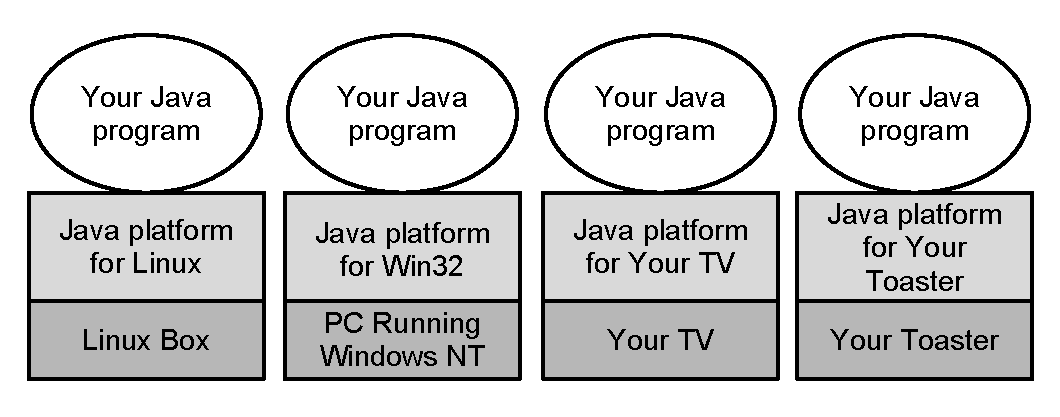
\includegraphics[width=\textwidth]{./images/java_platform.pdf}
  \caption{Java programs run on top of Java platform\cite{venners1996inside}.}
  \label{fig:figure2}
\end{figure}

To meet these requirements one needs tools that empowers developers to make portable programs. In other words, tool that meets the principle of \textbf{WORA} (Write Once Run Anywhere). The way to fulfill this principle is to use concept of virtual machines because it gives you an abstraction of an underlying platform. For example, if there is a need to support Java applications on one more hardware and OS platform, the only thing you need to do is to port JVM to that platform and existing applications will work on it. This is possible because JVM executes java byte code which stays hardware- and OS-independent. 

\subsection{Motivation for DVM}

As stated in Android homepage:
\begin{quotation}
Our primary purpose is to build an excellent software platform for everyday users\cite{website:androidphylosophy}.
\end{quotation}
To build such software platform one also needs a virtual machine because there are huge variety of devices that those ``everyday users'' have. There were many reasons that pushed Google to develop a custom clean-room virtual machine of their own rather than using one of the existing Java Virtual Machines and below we'll emphasize some of the most important.

\subsubsection{J2ME problems}

While Java technology adoption for desktops is more or less homogenous, for mobile platforms situation is not that attractive. In the days, when Android was just an idea, J2SE (Java 2 Standard Edition) for mobile devices was too ``heavy''. Lighter Java version -- J2ME (Java 2 Mobile Edition) -- was lacking in key features that are very important for modern smartphones such as Bluetooth support or 3D graphics were available only on subset of devices. Because of the presence of "Java Community Process" organization\cite{java_community_process}, to standardize J2ME would have been long and bureaucratic process. Also, a large part of the reason Java has had limited success in the past on mobile platforms is due to the speed of mobile Java platforms which are not designed to take advantage of today's smartphone devices. 

\subsubsection{Platform constraints}

Android is designed mainly for smartphones and tablets which are constrained by limited resources. Virtual machine that runs in those devices should address those constraints. DVM is designed to run in the device which has:
\begin{itemize}
\itemsep0em
  \item Slow CPU: 250-500 MHz;
  \item Relatively little amount of RAM: total ~64 MB, from which ~20 MB are available for applications;
  \item OS without swap space;
  \item Device is powered by a battery;
\end{itemize}
When compared to the desktops, these resources are very limited. So, there was a need to rethink the whole software stack and, at the same time, to find a VM solution for mobile platforms. 

\subsection{Comparison of key JVM and DVM motivations}

Common motivation for both JVM and DVM is that they are trying to address the problem of running software in heterogeneous platforms which are used by ``everyday users''.

Security is always important issue for information systems. It is widely known that VM technology provides isolation between multiple systems running concurrently on the same hardware platform\cite{smith2005architecture}.

The difference is that in DVM case, the platform is very resource constrained, when compared to the platform JVM is aiming to. 

\section{Architecture of virtual machines}

The term architecture is used here to describe the attributes of the system as seen by the programmer, i.e., \textbf{the conceptual structure and functional behavior}, as distinct from the organization of the data flow and controls, the logic design, and the physical implementation\cite{amdahl1964architecture}.

In this section we discuss what VM should implement. Furthermore, we take a brief look at architectural difference of system and process VM's. Also, we describe stack-based and registry-based VM's, the main differences between them, and the consequences of those differences.

\subsection{What should virtual machine implement?}

A virtual machine should emulate the operations carried out by a physical CPU and thus should ideally encompass the following concepts\cite{website:dalvikjit2010}:
\begin{itemize}
  \itemsep0pt
  \item Compilation of source language into VM specific byte code;
  \item Data structures to contain instructions and operands;
  \item A call stack for function call operands;
  \item An ``Instruction Pointer'' (IP) pointing to the next instruction to execute;
  \item A virtual CPU - the instruction dispatcher that:
  \begin{itemize}
    \item Fetches the next instruction (addressed by the instruction pointer);
    \item Decodes the operands
    \item Executes the instructions;
  \end{itemize}
\end{itemize}

%% In more detail we'll analyze what are the WHAT??? limitations of DVM comparing to JVM. Moreover, we'll discuss what is the typical programmer workflow of development for JVM and DVM.

\subsection{System and process VM's}

A system virtual machine provides a complete system platform which supports the execution of a complete operating system (OS). A process virtual machine (also, language virtual machine) is designed to run a single program, which means that it supports a single process\cite{wiki_vm}.

Conceptual difference between system and process VM's is shown in figure \ref{fig:system_and_process}. The main advantage of using process VM is that if a VM crashes the other processes are not affected.

Both JVM and DVM are process VM's. From this perspective JVM and DVM are similar.
\begin{figure}
  \center
  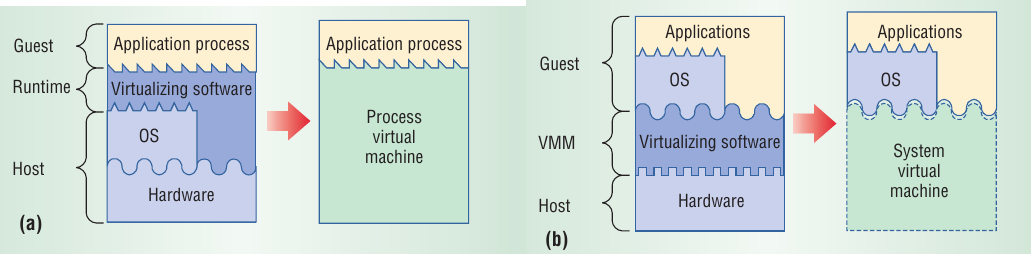
\includegraphics[width=\textwidth]{./images/vms.png}
  \caption{Conceptual architecture of system and process virtual machines\cite{smith2005architecture}. a)}
  \label{fig:system_and_process}
\end{figure}

\subsection{Stack-based VM's}

A stack-based VM implements  previously described concepts using the data structure of the stack for memory organization. In this data structure operands are stored. Operands are carried out by popping (POP) data from the stack, processing the popping out (POP) and pushing in (PUSH) back the result in LIFO (Last In First Out) fashion. 

The advantage of the stack based model is that the operands are addressed implicitly by the stack pointer (SP). This means that the VM does not need to know the operand addresses explicitly, as calling the stack pointer will give (POP) the next operand. In stack-based VM's, all the arithmetic and logic operations are carried via pushing and popping the operands and results in the stack.

In stack-based VM's adding two numbers usually is carried out in the following manner:
\begin{enumerate}
  \itemsep0pt
  \item POP 20
  \item POP 7
  \item ADD 20, 7, result
  \item PUSH result
\end{enumerate}
Illustration of addition process is in the figure \ref{fig:stackadd}.

\begin{figure}[h]
\centering
\begin{minipage}{.47\textwidth}
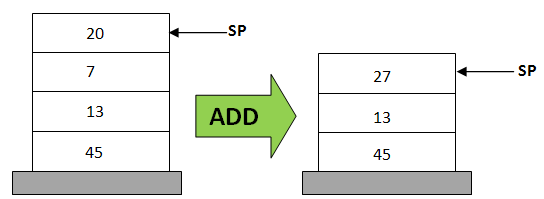
\includegraphics[width=0.8\textwidth]{./images/stackadd.png}
  \caption{Addition in stack-based VM architecture.}
  \label{fig:stackadd}
\end{minipage}
\begin{minipage}{.5\textwidth}
  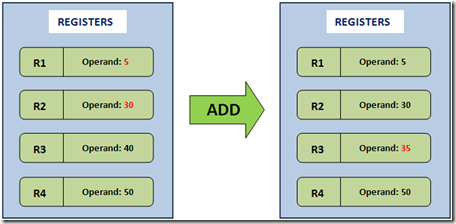
\includegraphics[width=0.8\textwidth]{./images/registeradd.png}
  \caption{Addition in register-based VM architecture.}
  \label{fig:registeradd}
\end{minipage}
\end{figure}


\subsection{Registry-based VM's}

In the register-based VM implementations, the data structure where operands are stored is based on the registers of the CPU. There is no PUSH or POP operations, therefore the instructions need to contain the addresses (the registers) of the operands. That is the operands for the instructions are explicitly addressed in the instruction, unlike the stack based model where we had a stack pointer (SP) to point to the operand. 

Compared to stack-based VM addition is just one operation: \textbf{ADD R1, R2, R3;}. Graphical interpretation of the register-based addition process is in the figure \ref{fig:registeradd}.

\subsection{Main advantages of register-based over stack-based VM's}

Main advantages of registry-based VMs compared to stack-based VMs that are important for mobile environments:
\begin{itemize}
  \itemsep0pt
  \item a register-based VM reduces the number of instructions to be executed, because one instruction is more expressive;
  \item the resulting executable code is larger, yet it requires less time to run;
  \item avoids instruction dispatch, because in gereral there are fewer instructions;
  \item avoids unnecessary memory access;
  \item consume instruction stream efficiently;
\end{itemize}

Generally speaking, the code size of register-based VM instructions are larger than that of the 
corresponding stack-based VM instructions. At the same time the instruction number is lower. It means that less CPU usage and then power saving. 

Having all operands in the instruction has its benefits; the execution is faster compared to the stack VM, which needs a small calculation to find out the operand, while register VMs just read the registers.

In register VMs, temporary values usually remain in registers. Stack VMs are unable to use a few optimisations too. For example, in the case of common sub-expressions, which are recalculated each time they appear in the code, a register VM can calculate an expression once, and keep that in a register for all future references.

Because code efficiency and power management is of a paramount importance for mobile environment, DVM was implemented as a registry-based VM.

\begin{comment}
$2^16$ registers,
218 opcodes (JVM 200 opcodes).

30\% fewer instructions, but 35\% larger code size 
(bytes) compared to JVM

\subsection{JIT}

Android needs a combination that meet the needs of a mobile 
- Minimal additional memory usage
- Coexist with Dalvik?s container-based security model
- Quick delivery of performance boost
- Smooth transition between interpretation \& compiled code

%%\subsection{Performance comparison}

\section{Code support}

\subsection{Architecture of JVM}

JVM operates on Java bytecode\cite{khan2009analysis}. The code written in Java programming language is executed by following the process shown in the figure \ref{fig:figure3}.
\begin{figure}
  \center
  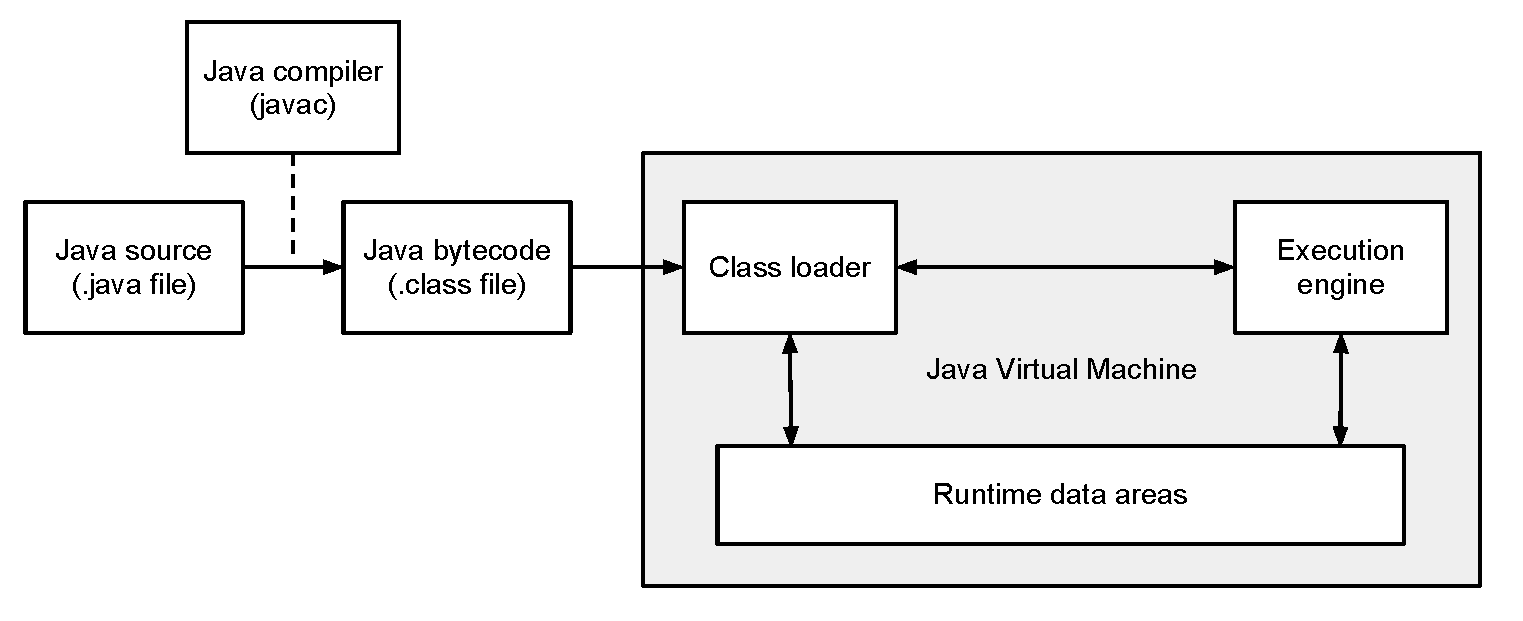
\includegraphics[width=\textwidth]{./images/java_code_execution_process_1.pdf}
  \caption{Java code execution process.}
  \label{fig:figure3}
\end{figure}
Java provides a dynamic load feature; it loads and links the class when it refers to a class for the first time at runtime, not at compile time. JVM's class loader executes the dynamic load.

\subsection{Architecture of DVM}

Compiling? Linking? Dynamic loading? How to run multiple VM's efficiently?
 \cite{wiki_dalvikvm}.

\subsection{Comparison of architectures}

\begin{figure}
  \center
  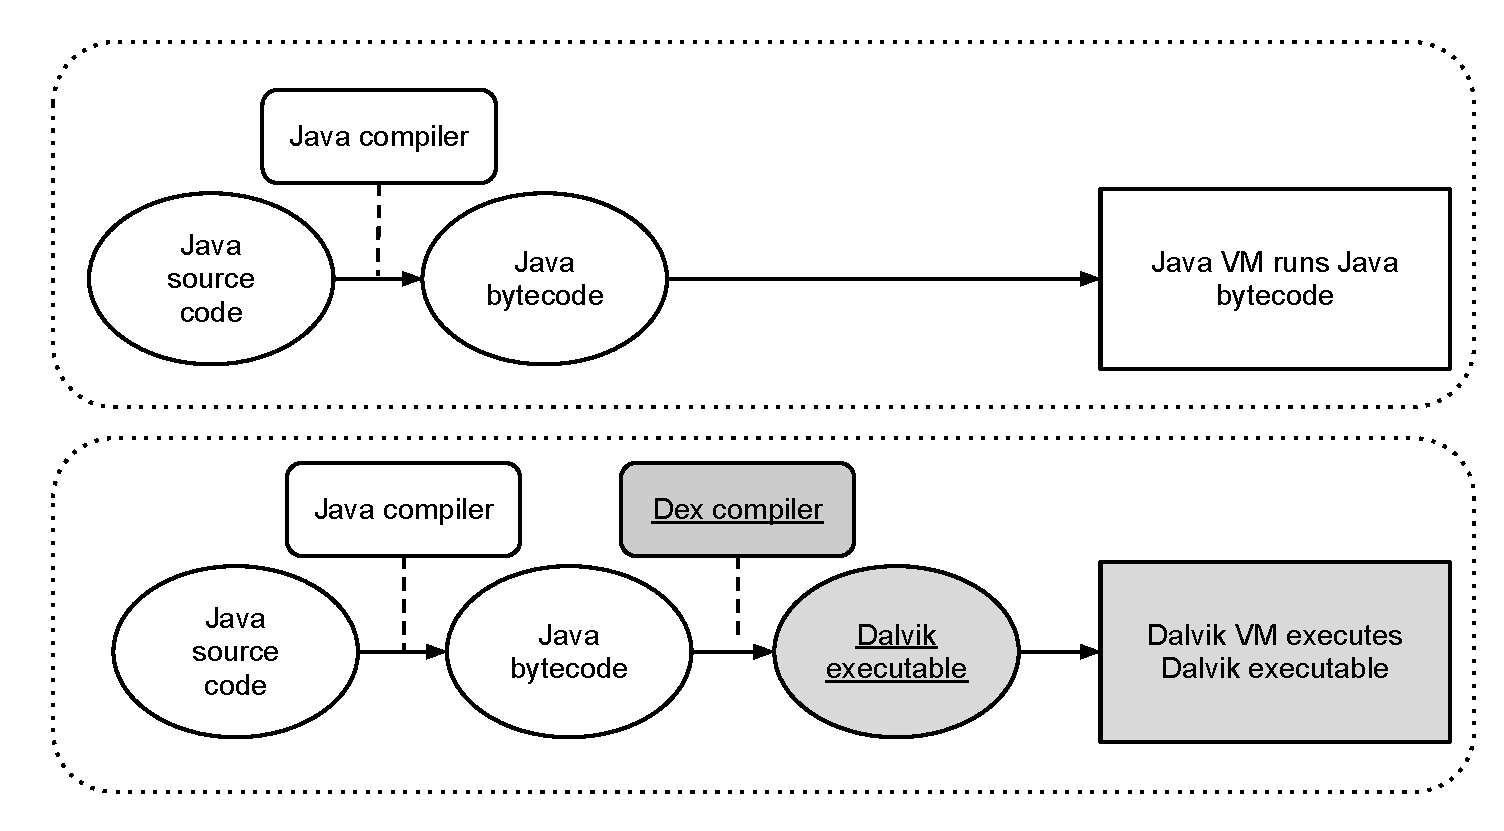
\includegraphics[width=\textwidth]{./images/jvm_vs_dvm.pdf}
  \caption{Typical application for JVM and DVM development workflows.}
  \label{fig:figure5}
\end{figure}
\end{comment}

\section{Executable format}

In this section we describe internal file structure of .class and .dex file formats. Also, we discover relation between the two file types. Moreover, we provide analysis of bytecode. 

\subsection{.class file structure}

In standard Java environments, Java source code is compiled into Java Bytecode, which is stored within .class files. The .class files are read by the JVM at runtime. Each class in your Java code will result in one .class file. This means that if you have, say, one .java source file that contains one public class, one static inner class, and three anonymous classes, the compilation process (javac) will output 5 .class files.

An internal structure of .class files\cite{dot_class_structure}:
\begin{itemize}
\itemsep0pt
  \item A header containing a ``magic number'' and a version number;
  \item A constant pool;
  \item Access rights of the class encoded by a bit mask;
  \item A list of interfaces implemented by the class;
  \item A list containing fields of the class;
  \item A list of methods of the class;
  \item A list of the class attributes (e.g. exceptions);
\end{itemize}

\begin{figure}[h]
\centering
\begin{minipage}{.4\textwidth}
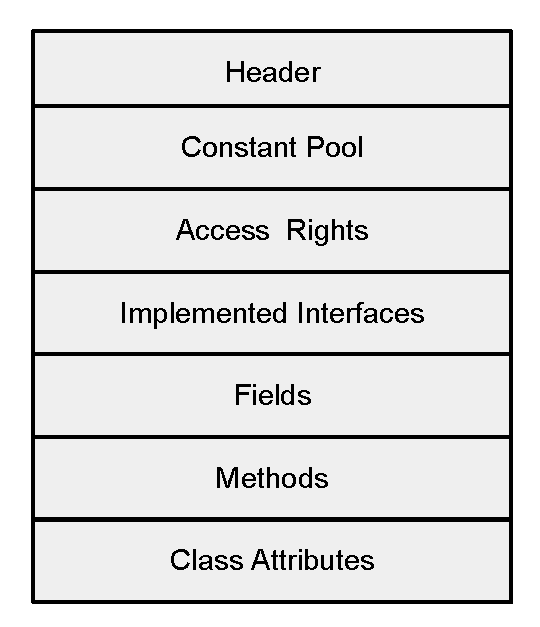
\includegraphics[width=\textwidth]{./images/dot_class_file_structure.pdf}
\caption{.class file logical structure.}
\label{fig:dot_class_internals}
\end{minipage}
\begin{minipage}{.45\textwidth}
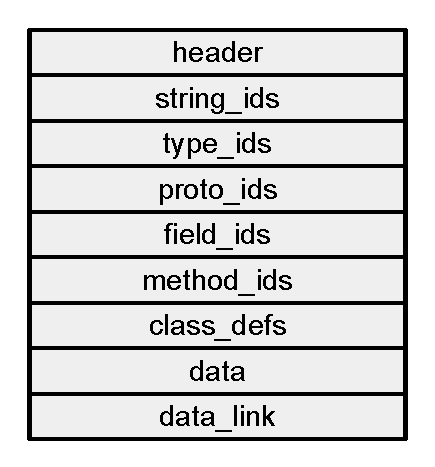
\includegraphics[width=\textwidth]{./images/dot_dex_file_structure.pdf}
\caption{.dex file logical structure.}
\label{fig:dex_structure}
\end{minipage}
\end{figure}

Typically .class files are distributed in collections. Those collections are .jar files. .jar files are nothing more than zipped collection of .class files.

\subsection{.dex file structure}

Bytecode for DVM is stored in .dex (Dalvik EXecutable) files. Bytecode for .dex files are generated from byte code stored .class files using the \textbf{dx} tool. The format of the .dex file is the following \cite{dot_dex_structure}:
\begin{itemize}
  \itemsep0pt
  \item Header with ``magic number'' and version number;
  \item A constant pool for each family of elements (strings, fields, methods...);
  \item Definition of classes;
  \item Definitions of methods;
  \item Reserved space for general data; 
\end{itemize} 

Dex file has a limitation of 64K method references. Usually, one Android application has one .dex file, which has all the necessary code. 
But sometimes, big applications can contain more than 64K method references. To get around this limitation, developers can partition part of the program into multiple secondary dex files, and load them at runtime.

\subsection{Relation between .dex and .class file types}

As stated before .dex files are compiled from .class files. This compilation takes all the needed .class files, analyzes them, optimizes the overall structure and puts everything into a .dex file. Basically, .dex file is an optimized collection of .class files, e.g. figure \ref{fig:class_dex}. These optimizations leads to a measurable savings in memory consumption. These saving are achieved due to the fact that .dex files avoid repetition of data, and implicit typing and implicit labeling are used.
\begin{figure}
  \center
  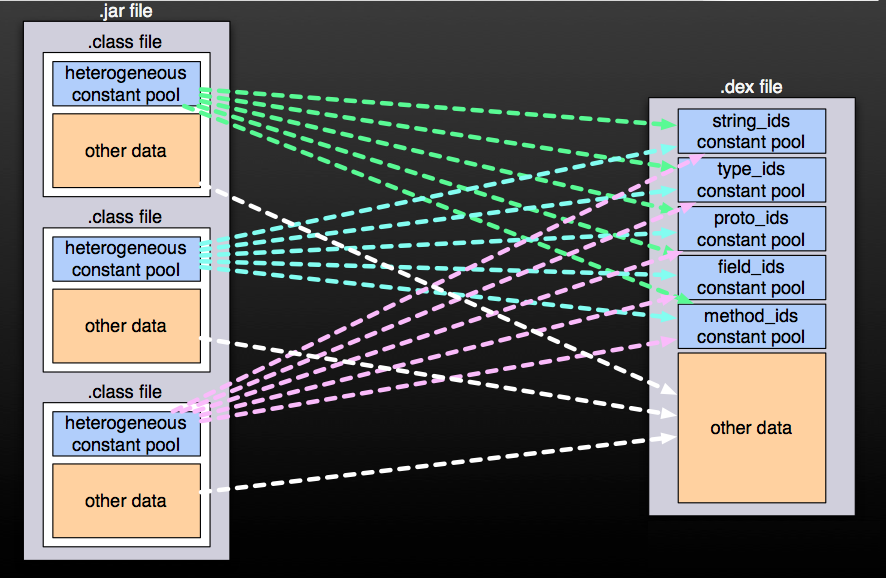
\includegraphics[width=0.9\textwidth]{./images/class_dex.png}
  \caption{.class files compiled into .dex file.}
  \label{fig:class_dex}
\end{figure}

Some of the optimizations done while constructing .dex files:
\begin{itemize}
 \itemsep0pt
 \item All separate constant pools are consolidated into one shared constant pool. Therefore, minimal repetition, per-type pools (implicit typing), implicit labeling.
 \item For instance field get/put, replace the field index with a byte offset. Also, merge the boolean / byte / char / short variants into a single 32-bit form (less code in the interpreter means more room in the CPU I-cache).
 \item Symbolic references from one class file to another are changed to static pointers.
 \item Inlining special native methods, e.g. String.length().
 \item Byte-swapping and padding.
 \item Pruning empty methods.
 \item Adding auxiliary data, e.g. a hash table for lookups on class name.
\end{itemize}


\subsection{Bytecode differences}

The most dignificant differences between JVM and DVM bytecode:
\begin{itemize}
 \itemsep0pt
 \item Code unit in JVM is one byte, Dalvik - 2 bytes.
 \item DVM has 230 opcodes while JVM has 225 different opcodes.
 \item In JVM, the opcodes for integers and single float constants are different, along with long integers and double float constants. While Dalvik implements the same opcode for both, integers and float constants.
 \item Dalvik bytecode does not have a specific null type. Instead, Dalvik uses a 0 value constant. So, the ambiguous implication of constant 0 should be distinguished properly.
 \item JVM bytecode uses different opcodes for object reference comparison and null type comparison, while Dalvik simplifies them into one opcode. Thus, the type info of the comparison object must be recovered during decompilation.
\end{itemize}

\section{Code support}

Usually applications for Android OS are written in Java programming language. Android API supports a relatively large subset if Java Standart Edition 5.0 library but some libraries are left out. Some things were left out because they simply didn’t make sense (like printing), and others because better APIs are available that are specific to Android (like user interfaces). 

In this section we take a look at which libraries are left out of Standard Java API. Also, we briefly describe what are spiceific Java libraries for android.

\subsection{Standard Java API libraries that are not supported in Android}

\begin{longtable}{| p{5cm} | p{10cm} |}
\caption{Libraries from Java API that are not supported in Android API\label{table:comparison}}\\
%% header for the first page table
\hline \hline
{\textbf{Library}} &
{\textbf{Comment}} \\
\hline
\endfirsthead

%% header for remaining pages
\multicolumn{2}{c}{{\tablename} \thetable{} -- Continued} \\[0.5ex]
\hline \hline
{\textbf{Library}} &
{\textbf{Comment}} \\
\hline
\endhead
\multicolumn{2}{l}{{Table continues on the next page\ldots}} \\
\endfoot
\hline \hline
\endlastfoot

%%\begin{tabular}{| l | l | l | l |}
\hline
java.applet & Provides the classes necessary to create an applet and the classes an applet uses to communicate with its applet context.
\\ \hline
java.awt & Contains all of the classes for creating user interfaces and for painting graphics and images.
\\ \hline
java.beans & Contains classes related to developing beans -- components based on the JavaBeansTM architecture.
\\ \hline
java.lang.management & Provides the management interface for monitoring and management of the Java virtual machine as well as the operating system on which the Java virtual machine is running.
\\ \hline
java.rmi & Java Remote Method Invocation (Java RMI) enables the programmer to create distributed Java technology-based to Java technology-based applications, in which the methods of remote Java objects can be invoked from other Java virtual machines*, possibly on different hosts.
\\ \hline
javax.accessibility & Defines a contract between user-interface components and an assistive technology that provides access to those components.
\\ \hline
javax.activity & Contains Activity service related exceptions thrown by the ORB machinery during unmarshalling.
\\ \hline
javax.imageio & The main package of the Java Image I/O API.
\\ \hline
javax.management & Provides the core classes for the Java Management Extensions.
\\ \hline
javax.naming & Provides the classes and interfaces for accessing naming services.
\\ \hline
javax.print & Provides the principal classes and interfaces for the JavaTM Print Service API.
\\ \hline
javax.rmi & Contains user APIs for RMI-IIOP.
\\ \hline
javax.security.auth.kerberos & This package contains utility classes related to the Kerberos network authentication protocol.
\\ \hline
javax.security.auth.spi & This package provides the interface to be used for implementing pluggable authentication modules.
\\ \hline
javax.security.sasl & Contains class and interfaces for supporting SASL.
\\ \hline
javax.swing & Provides a set of "lightweight" (all-Java language) components that, to the maximum degree possible, work the same on all platforms.
\\ \hline
javax.transaction & Provides the API that defines the contract between the transaction manager and the various parties involved in a distributed transaction namely : resource manager, application, and application server.
\\ \hline
javax.xml (except javax.xml.parsers) & This package contains the core JAX-WS APIs.
\\ \hline
org.ietf.* & This package presents a framework that allows application developers to make use of security services like authentication, data integrity and data confidentiality from a variety of underlying security mechanisms like Kerberos, using a unified API.
\\ \hline
org.omg.* & Provides the mapping of the OMG CORBA APIs to the JavaTM programming language, including the class ORB, which is implemented so that a programmer can use it as a fully-functional Object Request Broker (ORB).
\\ \hline
org.w3c.dom.* (sub-packages) & Provides the interfaces for the Document Object Model (DOM) which is a component API of the Java API for XML Processing.
\\ \hline
\end{longtable}

\subsection{Android specific libraries}

In this section we'll take a look which standard Java libraries are unavailable to use in DVM and which libraries are specific to DVM are unavailable to use in JVM.


\section{Just-In-Time Compilation}

Just-in-time compilation (JIT), also known as dynamic translation, is a method to improve the runtime performance of computer programs based on bytecode (virtual machine code). It works translating the original bytecode to the native code, e.g. Java bytecode to assembly code. 

In this section we describe JVM relationship with JIT and DVM approach to JIT.

\subsection{JVM and JIT}

On a Java virtual machine implemented in software, the simplest kind of execution engine just interprets the bytecodes one at a time. Another kind of execution engine, one that is faster but requires more memory, is a just-in-time compiler. In this scheme, the bytecodes of a method are compiled to native machine code the first time the method is invoked. The native machine code for the method is then cached, so it can be re-used the next time that same method is invoked. A third type of execution engine is an adaptive optimizer. In this approach, the virtual machine starts by interpreting bytecodes, but monitors the activity of the running program and identifies the most heavily used areas of code. As the program runs, the virtual machine compiles to native and optimizes just these heavily used areas. The rest of the of code, which is not heavily used, remain as bytecodes which the virtual machine continues to interpret. 

\subsection{DVM and JIT}

In Android OS lots of native code does the ``heavy lifting'' (e.g. graphics, media) out of the box. Also, JNI is available for developers to speed up their applcations. On the other hand, while developing for Android OS it is unavoidable to use Java API. So, in some applications JIT can significantly increase execution speed. It is important to mention that JIT doesn't improve speed if code already is doing work in native code.

One of the most important requirement for DVM is to use small amount of RAM. Therefore, light usage of memory is very important for DVM JIT design. In order to reduce memory usage, DVM use a trace-based JIT compilation approach -- detects what are the hottest parts of code and compiles it into native code. 

Since JIT at runtime increases system load and therefore battery usage, DVM JIT compiler does a lot of work upfront run time, in order to be fast at run time. Some optimizationsare done on the development PC which has more power available. Also, some compilation are performed while device is charging.


\section{Conclusion}

The Dalvik VM has technical advantages over the Java VM for mobile environments, most notably aggressive use of copy-on-write memory sharing, so the entire VM and standard class library is shared among all Android SDK app processes, reducing the net per-process memory footprint.


\bibliographystyle{plain}
\bibliography{literature}

\begin{comment}
\section{Definitions}

\begin{description}
  \item[Java technology] Java technology is both a programming language and a platform.
  \item[Java Platform] A platform is the hardware or software environment in which a program runs. Java platform is software only platform which has two components: The Java Virtual Machine and The Java Application Programming Interface (API)\cite{website:javadefinitions}.
\end{description}
\end{comment}

\appendix
\section{Comparison of JVM and DVM}

\begin{longtable}{| p{3cm} | p{2cm} | p{2cm} | p{7cm} |}
\caption{Main features of JVM and DVM.\label{table:comparison}}\\
%% header for the first page table
\hline \hline
{\textbf{Feature}} &
{\textbf{JVM}} &
{\textbf{DVM}} &
{\textbf{Note}} \\
\hline
\endfirsthead

%% header for remaining pages
\multicolumn{3}{c}{{\tablename} \thetable{} -- Continued} \\[0.5ex]
\hline \hline
{\textbf{Feature}} &
{\textbf{JVM}} &
{\textbf{DVM}} &
{\textbf{Note}} \\
\hline
\endhead
\multicolumn{3}{l}{{Table continues on the next page\ldots}} \\
\endfoot
\hline \hline
\endlastfoot

%%\begin{tabular}{| l | l | l | l |}
\hline
JIT
&
+
&
+
& In Dalvik JIT was introduced in Android 2.2
\\ \hline
Bytecode	
&
javac
& 
Dalvik VM specifi
& .class files recompiled with dx tool
\\ \hline
Size of VM instructions
&
1 byte
&
2 Bytes
&
Increased expressiveness
\\ \hline
Method references
&
No limit
&
65536
&
It is possible to load multiple dec files into environment, but is important only for really huge apps 
\\ \hline
where is code?
&
Multiple .class files
&
one .dex file
&
There is a trick to have few dec files.*
\\ \hline
Memory consumption
&
Separate JVM, a lot of Ram
&
Shared libraries, small amount of ram
&
Dalvik is optimized for constraints
\\ \hline
Security
&
In one VM every app can access everything
&
Separate VMs
&
very good
\\
\hline
\end{longtable}

\begin{comment}
\section{Information sources}

The famous Dalvik introduction talk: 
http://www.youtube.com/watch?v=ptjedOZEXPM

http://www.artima.com/insidejvm/ed2/introarch.html

http://stackoverflow.com/questions/11374477/android-javac-vs-dalvik

http://android-developers.blogspot.it/2011/07/custom-class-loading-in-dalvik.html

http://blog.davidehringer.com/tag/jvm/

http://android-developers.blogspot.it/2010/05/dalvik-jit.html

http://jaxenter.com/android-dalvik-virtual-machine-35498.html

http://source.android.com/tech/dalvik/instruction-formats.html

TODO:

http://code.google.com/p/android/issues/list?q=label:Component-Dalvik

http://source.android.com/tech/dalvik/instruction-formats.html

http://jaxenter.com/android-dalvik-virtual-machine-35498.html

http://www.artima.com/insidejvm/ed2/jvm.html

http://www.artima.com/insidejvm/ed2/platindep.html

http://www.cubrid.org/blog/dev-platform/understanding-jvm-internals/

http://www.artima.com/underthehood/index.html

http://www.slideshare.net/dougqh/inside-androids-dalvik-vm-nejug-nov-2011
\end{comment}

\end{document}
